\documentclass[12pt,oneside,final]{book}
%\documentclass[12pt,A4,oneside,final]{book}

% \usepackage[portuguese,brazil]{babel}
 %\usepackage[latin1]{inputenc}

\usepackage[utf8]{inputenc}
 \usepackage[portuguese,brazil]{babel}

% Codificação da fonte
%\usepackage[T1]{fontenc}

%\usepackage[brazilian]{babel}
%\usepackage{graphicx}
\usepackage{subfigure}
\usepackage{colortbl}
\usepackage{cancel}
%**********************

\usepackage{indentfirst}
\usepackage{ae}
\usepackage{harvard}
\usepackage{amssymb,fancyhdr,fancybox,epsfig,psfrag,amsmath,tabularx}
\usepackage[paperwidth=8.5in,paperheight=11in,hmargin={25mm,20mm},vmargin={20mm,20mm}]{geometry} %tamanho letter



\usepackage[color]{showkeys}
\definecolor{refkey}{rgb}{0.39,0.58,1}
\definecolor{labeled}{rgb}{1,0,0}
\usepackage[Lenny]{fncychap}
\setlength{\headheight}{15pt}

%=========================================== Headers ===============================================
\renewcommand{\chaptermark}[1]{\markboth{\chaptername\ \thechapter. \ #1}{ }}
\renewcommand{\sectionmark}[1]{\markright{\thesection. \ #1}}
\fancyhead{}
\fancyfoot{}
\fancyhead[LO]{\nouppercase{\leftmark}}
\fancyhead[RO]{\thepage}

% Espacos H2, Hoo, L2, Loo
\newcommand\Hi{{\mathcal{H}}_{\infty}}
\newcommand\Hd{{\mathcal{H}}_{2}}
\newcommand\Li{{\mathcal{L}}_{\infty}}
\newcommand\Ld{{\mathcal{L}}_{2}}


\def\reais{{\rm I\kern-.17em R}} % R de reais
\def\Dest{{\rm I\kern-.17em D}} % R de reais
\newcommand{\Dgest}{\ensuremath{\mathcal{D}}}
\newcommand{\naturais}{\mathbb{N}}
\newcommand{\inteiros}{\mathbb{Z}_{+}}
\newcommand{\matlab}{{\sc Matlab}}

%super parenteses
\makeatletter
\def\Biggg#1{{\hbox{$\left#1\vbox to29\p@{}\right.\n@space$}}}
\newdimen\bracketwidth
\settowidth{\bracketwidth}{\Biggg(} \makeatother


%\newcommand{\carinha}{\raisebox{-.2ex}{\epsfxsize 3mm \epsffile{cara.eps}}}

% Bolds
\newcommand{\I}{{\bf I}}
\newcommand{\Z}{{\bf 0}}
\newcommand{\Bfres}{\mathcal{B}}

% funcoes
\newcommand{\Tr}{\mbox{Tr}}

% Referencia com parenteses
\newcommand{\bref}[1]{\mbox{(\ref{#1})}}

% Ambiente de equacoes
\newcommand\be{\begin{equation}}
\newcommand\ee{\end{equation}}
\newcommand\vi{\vspace{\baselineskip}}

% newtheorems e similares

\newtheorem{teorema}{\noindent{\bf Teorema} }[chapter]
\newtheorem{lema}{\noindent{\bf Lema} }[chapter]
\newtheorem{corolario}{\noindent{\bf Corol�rio} }[chapter]
\newenvironment{prova}{\noindent{\bf Prova:}}{\null\hfill $\rule{1.5mm}{1.5mm}$}
\newtheorem{definicao}{\noindent{\bf Defini��o} }[chapter]

\newcommand{\simplex}{\Delta_N}



\newcommand{\Aal}{A(\alpha)}
\newcommand{\Bal}{B(\alpha)}
\newcommand{\Cal}{C(\alpha)}
\newcommand{\Dal}{D(\alpha)}


\newcommand{\Pal}{P(\alpha)}
\newcommand{\Gal}{G(\alpha)}
\newcommand{\Hal}{H(\alpha)}
\newcommand{\Qal}{Q(\alpha)}
\newcommand{\Xal}{X(\alpha)}
\newcommand{\Xual}{X_1(\alpha)}
\newcommand{\Xdal}{X_2(\alpha)}

\newcommand{\Sfr}{\mathcal{S}}

\newcommand{\Xfal}{\mathcal{X}(\alpha)}
\newcommand{\Bfal}{\mathcal{B}(\alpha)}
\newcommand{\Qfal}{\mathcal{Q}(\alpha)}
\newcommand{\Sfal}{\mathcal{S}(\alpha)}

\newcommand{\Kfr}{\mathcal{K}}
\newcommand{\Ifr}{\mathcal{I}}
\newcommand{\Afr}{\mathcal{A}}
\newcommand{\Pfr}{\mathcal{P}}
\newcommand{\Cfr}{\mathcal{C}}
\newcommand{\Gfr}{\mathcal{G}}


\begin{document}

\pagenumbering{roman}
\pagestyle{plain}

%Tese em português
%=========================================================
%                                                       PRIMEIRA FOLHA INTERNA  %=========================================================
\begin{figure}
    
\includegraphics[width=0.12\textwidth]{./eps/unicamp}
\end{figure}


\vspace*{2.0cm}
\begin{center}
\large ROGER LEONARDO GARAY AVENDAÑO
\end{center}


\vspace*{3.8cm} % 6.8

\begin{center}
{\sc \large  FORMULAÇÃO ANALÍTICA EXATA DE FEIXES ELETROMAGNÉTICOS NÃO PARAXIAIS}
\end{center}


\vspace*{3.25cm}


\null \vfill

\begin{center}
CAMPINAS\\2013
\end{center}
\thispagestyle{empty}
\newpage

%==========================================================
%                                                           FOLHA DE ROSTO %==========================================================
\pagenumbering{roman}
\pagestyle{plain}
\begin{figure}
    
\includegraphics[width=0.12\textwidth]{./eps/unicamp}
\end{figure}

\begin{center}
\large Universidade Estadual de Campinas\\
Faculdade de Engenharia Elétrica e de Computação
\end{center}

\vspace*{1.5cm}
\begin{center}
\large ROGER LEONARDO GARAY AVENDAÑO
\end{center}

\vspace*{1.3cm}

\begin{center}
{\sc \large FORMULAÇÃO ANALÍTICA EXATA\\
 DE FEIXES ELETROMAGNÉTICOS NÃO PARAXIAIS}
\end{center}


\vspace*{1.3cm}

{\bf Orientador: Prof. Dr. Michel Zamboni Rached}


\vspace*{1.0cm} % 3.0

\begin{flushright}
\begin{minipage}{9.0cm}
Qualificação de Doutorado apresentada ao Programa de Pós-Graduação em Engenharia Elétrica da Faculdade de Engenharia Elétrica e de Computação da Universidade Estadual de Campinas para obtenção do título de Doutor em Engenharia Elétrica, na Área de Concentração: AG.

%Dissertação de Mestrado apresentada ao Programa de Pós-Graduação em Engenharia Elétrica da Faculdade de Engenharia Elétrica e de Computação da Universidade Estadual de Campinas para obtenção do título de Mestre em Engenharia Elétrica, na Área de Concentração: AG.

\end{minipage}
\end{flushright}

\null \vfill
\begin{minipage}{7cm}
\small
%Este exemplar corresponde à versão final da dissertação defendida pelo
%aluno Roger Leonardo Garay Avendaño, e orientada pelo Prof. Dr. Michel Zamboni Rached\\[4mm]
%\rule{7.0cm}{0.2mm} \hfill
\end{minipage}

\vspace*{0.9cm} %0.5

\begin{center}
CAMPINAS\\2013
\end{center}

%\null \vfill
%\newpage
%=================================================
%                                                  Ficha (Somente na versao final) %=================================================


%\begin{center}

%\begin{figure}
    %\includegraphics[width=1.0\textwidth]{./eps/FichaCatalografica1}
%\end{figure}

%\end{center}



%=====================================================
%                        Folha de aprovacao (Somente depois da defensa) %======================================================


%\begin{center}
% conveniente scanear o documento e convertir-lo para o formato .png. 
%\begin{figure}
    %\includegraphics[width=1.1\textwidth]{./eps/rogerbanca}
%\end{figure}
%\end{center}


%Tese em portugês e ingles
%\input{capaPortIngles}
%%======================================== Dedicat�ria =========================================
\null\vfill
\begin{flushright}
\begin{minipage}{6.5cm}
{\sc A Yuliana, meu amor}
\end{minipage} \\[8mm]
\end{flushright}
\null
%==============================================================================================

%
% ********** Agradecimentos
\chapter*{\centering{Agradecimentos}}


\begin{trivlist}  \itemsep 2ex  \normalsize

\item Agradeço primeiramente a Deus por toda a minha vida, pois sei que tudo o que ocorreu de bom em minha vida foi Ele que me presenteou.

\item À minha família, em especial meus pais, Leonardo e Reneé, e a minha irmã Katherine que nunca hesitaram em me apoiar, tanto financeiramente como afetivamente. Sempre os amarei.

\item À minha noiva, Yuliana, que sem sua paciência e compreensão esse trabalho não ficaria pronto. Agradeço pelo incentivo através de palavras e exemplo, que sempre me deu. Agradeço por estar comigo por todo esse tempo, e ainda rezo para que possamos continuar juntos por toda as nossas vidas. Te amo muito!

\item Ao meu orientador, Prof. Dr. Michel Zamboni Rached, sou grato pela orientação prestada, pela virtuosa compreensão em tudo, pelo seu incentivo, disponibilidade e apoio que sempre demonstrou.

\item Aos amigos, brasileiros, cubanos, argentinos e peruanos da Sala $3$ e Sala $4$, sou grato pelas horas de descontração em meio a tanto trabalho. Em especial ao Iury - pela paciência em ensinar-me "engenheirês", a Ruthy e Yuri - pelo grande apoio no decorrer deste mestrado, e a Mariana e Aleixo - pela companhia ao trilharmos o mesmo caminho.

\item Ao grande amigo Prof. Dr. Hugo E. H. Figueroa, pelo recebimento e a oportunidade a este grande mundo da pós graduação.

\item Á grande amiga Prof. Dra. Carmen Eyzaguirre, a qual me iniciou na vida acadêmica com muita paciência em repetitivas explicações. Obrigado pelos ensinamentos.

\item Sou grato também ao CAPES pelo financiamento.

\item A todos o meu sincero e profundo {\bf Muito Obrigado!}

\end{trivlist}



%% ********** Dedicatória - Back Page
\newpage \thispagestyle{plain}


%%======================================== Frase Miss Brasil ===================================
\newpage
\null\vfill
\begin{flushright}
\begin{minipage}{9.0cm}
Quem sabe concentrar-se numa coisa e insistir nela como único objetivo, obtém, ao fim e ao cabo, a capacidade de fazer qualquer coisa.
\end{minipage}
\end{flushright}


\begin{flushright}
 Mahatma Gandhi
\end{flushright}

\null
%==============================================================================================



\baselineskip 1.1 \baselineskip

%\input{res_abstract}


%=============================== lista de tabelas e figuras ===========================
\listoffigures

\listoftables

%============================ acrônimos, símbolos e notações =====================================
%%============================Acrônimos e Notação =================================================

\chapter*{Lista de Acrônimos e Notação}

\begin{tabular}{ll}
TE  & Transversal Elétrico\\
TM & Transversal Magnético\\
%LMI  & Linear Matrix Inequality (desigualdade matricial linear)\\
%LFT  & Linear Fractional Transformation (transformação linear fracionária)\\
%LPV  & Linear Parameter-Varying (linear com parâmetros variantes)\\
%IQC  & Integral Quadratic Constraint (restrição de integral quadrática)\\
\end{tabular}

\vspace*{1cm}

\begin{tabular}{ll}
$1D, 2D, 3D$ & indica dimensão espacial\\
$ x, y, z$ & variáveis espaciais cartesianas\\
$ \rho, \phi, z$ & variáveis espaciais cilíndricas\\
$\lambda$ & comprimento de onda no vácuo\\
$\omega$ & frequência angular de onda no vácuo\\
$c$ & velocidade da luz no vácuo\\
$J_0$ & função de Bessel de ordem zero\\
$J_{\nu}$ & função de Bessel de ordem$-\nu$\\
%$\star$ & indica bloco simétrico nas LMIs\\
%$L > 0$ & indica que a matriz $L$ é simétrica definida positiva\\
%$L \geq 0$ & indica que a matriz $L$ é simétrica semi-definida positiva\\
%$A$ & notação para matrizes (letras maiúsculas do alfabeto latino)\\
%$A'$ & ($'$), pós-posto a um vetor ou matriz, indica a operação de transposição\\
%$\reais$ & conjunto dos números reais\\
%$\mathbb{Z}$ & conjunto dos números inteiros\\
%$\mathbb{Z}_+$ & conjunto dos números inteiros não negativos\\
%$\mathbb{N}$ & conjunto dos números naturais (incluindo o zero)\\
%$\I$ & matriz identidade de dimensão apropriada\\
%$\Z$ & matriz de zeros de dimensão apropriada\\
%$g!$ & símbolo (!), denota fatorial, isto é, $g!=g (g-1) \cdots (2) (1)$ para $g \in \mathbb{N}$\\
$R_n$ & n-ésimo coeficientes de Fourier\\
$2N+1$ & número de coeficientes de Fourier\\
$k_{\rho}$ & componente transversal do vetor de onda\\
$k_{z}$ & componente longitudinal do vetor de onda\\
$S(k_z)$ & espectro em $k_z$\\
$\Delta k_z$ & largura de banda do espectro $S(k_z)$\\
$\bar{k}_{z}$ & posição do centro do espectro $S(k_z)$\\
$\Re e$ & parte real\\
$E_m$ & componentes do campo elétrico do modo $TM$\\
$B_m$ & componentes do campo magnético do modo $TM$\\
$E_e$ & componentes do campo elétrico do modo $TE$\\
$B_e$ & componentes do campo magnético do modo $TE$\\

%$n$ & especialmente utilizada para representar a ordem uma matriz quadrada\\
%$\simplex$ & simplex unitário de $N$ variáveis\\
%$\alpha$ & especialmente utilizada para representar as incertezas de um sistema
\end{tabular}

%==============================================================================================


%=============================== sumário ========================================================
\tableofcontents


\pagestyle{fancy}

\markboth{Introdução Geral}{Introdução Geral}
\chapter{Introdução Geral}
\pagenumbering{arabic}

Nesta seção apresentamos  uma revisão bibliográfica resumida, os objetivos e as justificativas  de nosso projeto.
\section{Revisão bibliográfica resumida}
Um feixe é uma solução monocromática da equação de onda que possui concentração transversal de campo. No caso escalar essas soluções são soluções da equação de onda e no caso vetorial essas soluções são soluções das equações de Maxwell.\\
Um feixe óptico pode ser construído a partir de superposições de ondas planas que se propagam em diferentes direções, sendo que o feixe óptico mais comum é o gaussiano.\\
Na atualidade o estudo de feixes ópticos vem apresentando uma grande demanda (teórica e prática), atingindo as mais diversas áreas, como em pinças ópticas 
%****************************************************************************************************************
%****************************************************************************************************************
\section{Objetivos e justificativas}
Este trabalho tem por objetivo geral desenvolver um método teórico capaz de fornecer feixes escalares e vetoriais propagantes não paraxiais com simetria azimutal como soluções analíticas exatas da equação de onda e das equações de Maxwell respectivamente. Feixes escalares propagantes não paraxiais sem simetria azimutal também são estudados como soluções analíticas exatas da equação de onda.\\
Este trabalho tem como objetivos:
\begin{itemize}
\item Adquirir conhecimento dos feixes escalares propagantes não paraxiais com simetria azimutal construídos como superposições de feixes de Bessel de ordem zero através de uma integração na componente longitudinal do vetor de onda $k_z$ com uma dada função espectral $S(k_z)$.
\item Usar o método matemático proposto em  para obter feixes escalares propagantes com simetria azimutal paraxiais e não paraxiais a partir de funções de espectro paraxial e não paraxial. Analisar espectros de tipo exponencial, quadrado e gaussiano. Aplicar o método matemático proposto em  para construir feixes escalares não propagantes sim simetria azimutal. 
\item Propor métodos matemáticos para a construção de feixes vetoriais propagantes não paraxiais simétricos como soluções analíticas exatas das equações de Maxwell. Estudo das polarizações dos feixes vetoriais em coordenadas cartesianas e cilíndricas.
\end{itemize}  
Dentro das justificativas podemos destacar que o estudo de feixes ópticos nos últimos anos vem apresentando uma grande demanda (teórica e prática) principalmente na construção de novos tipos de feixes, os quais possuem propriedades muito mais interessantes que os já conhecidos feixes gaussianos, como as aplicações em fibra óptica, guiamento óptico de átomos, alinhamento óptico, aplicações médicas, comunicações ópticas no espaço livre, aplicações em óptica não linear, etc. O estudo da propagação de feixes é realizado, em geral, a partir das soluções da equação de onda. Na atualidade soluções analíticas exatas da equação de onda descrevendo feixes são muito raras, por isso muita atenção é dada ao regime de propagação paraxial na obtenção de soluções analíticas e também numéricas.\\
Porém obter um método que forneça soluções analíticas exatas da equação de onda no regime não paraxial é de grande importância, pois poderemos tratar situações que não podem ser descritas por aproximações usuais.\\
Dentro das justificativas podemos destacar também que nosso método \cite{Stratton:02} distingue-se dos outros métodos em dois principais características: A primeira é que nosso método pode ser aplicado para qualquer tipo de feixe e não s\'o para um determinado feixe, como em \cite{Stratton:02, Jackson:03,Figueroa:05,Sochacki:1}.
  
************************************** 
 %c Introdução
%------------------------------
\chapter{Preliminares e Defini\c{c}\~{o}es}
\section{Feixes puramente propagantes com simetria azimutal}
Um feixe de Bessel com simetria axial \'e escrito como:
 \begin{equation}\label{eqA1}
    \psi(\rho,z,t)= J_0(k_\rho\rho)\exp[{-\rm i}k_z]\exp[{-\rm i}\omega t]
\end{equation}
com
\begin{equation}\label{eqA2}
    \frac{\omega^2}{c^2}= k^2_{\rho} + k^2_{z}
\end{equation}
onde $c$, $\omega$, $k_{\rho}$, $k_{z}$ são a velocidade da luz no vácuo, a frequência angular, o número de onda transversal e longitudinal, respetivamente.\\
Um feixe com simetria azimutal pode ser escrito como  uma superposição de feixes de Bessel de ordem zero ($J_0$) através de uma integração na componente transversal do vetor de onda $ k_{{\rho}} $ com uma função espectral $S_{\pm}^{'}(k_{\rho})$ %\cite{Lya:92}.
\begin{equation}\label{eqA3}
\psi(\rho,z,t)=
\int_{0}^{\omega/c}J_0(k_{\rho}\rho)\exp[\pm{\rm i}z\sqrt{\omega^2/c^2-k^{2}_{\rho}}]
\exp[{-\rm i}\omega t]S_{\pm}^{'}(k_{\rho})k_{\rho}dk_{\rho}d\omega
\end{equation}
 onde consideraremos $0\leq k_z\leq \omega /c$ para evitar componentes evanescentes.\\
Mediante o vínculo (\ref{eqA2}), podemos obter os feixes dados por (\ref{eqA3}) através de uma superposição em $k_z$:
\begin{equation}\label{eqA4}
\psi(\rho,z,t)=
\exp[{-\rm i}\omega t]\int_{-\omega/c}^{\omega/c}J_0(\rho\sqrt{\omega^2/c^2-k^{2}_{z}})\exp[{\rm i}k_z z]S(k_{z})dk_{z}
\end{equation} 
A superposição dada em (\ref{eqA4}) possui componentes propagantes e contra propagantes.
%***********************************************************************************************************************
\subsection{Feixes paraxiais e n\~ao paraxiais}
Na solução integral (\ref{eqA4}) o espectro de $S(k_z)$ define o tipo de feixe resultante. Feixes paraxiais são aqueles onde os espectros $S(k_z)$ são concentrados ao redor de $k_z = \omega /c$, com $\Delta k_z \ll \omega /c$. Algumas soluções de feixes paraxiais (como a tradicional solução do feixe gaussiano) podem ser obtidas analiticamente através da aproximação paraxial  \cite{Lya:3} \cite{Lya:4}\cite{Lya:12}, nesse caso o uso da solução (\ref{eqA3}) é mais indicada.\\
Feixes n\~ao paraxiais (puramente propagantes) s\~ao caracterizados por espectros de $S(k_z)$ de grande largura de banda; ou mesmo estreitos, por\'em concentrados em valores de $\bar{k}_z$ bem afastados do valor $k_z = \omega /c$.\\
Obter soluções analíticas exatas para feixes não paraxiais \'e um desafio devido à complexidade da integral (\ref{eqA4}). A seguir iremos expor o método capaz de solucionar (\ref{eqA4}) para qualquer espectro $S(k_z)$ e, portanto, capaz de fornecer soluções analíticas exatas descrevendo feixes não paraxiais (e também paraxiais) puramente propagantes. 
%***********************************************************************************************************************
\section{Metodologia matem\'atica para a construção de feixes escalares } 	
A demostração da metodologia matemática proposta, capaz de fornecer soluções analíticas exatas da equação de onda para qualquer espectro $S(k_z)$, \'e dividida em três passos. 
\subsection{Passo 1}
Primeiro consideramos um espectro constante:
\begin{equation}\label{eqA5}
    S(k_{z})=\frac{1}{2}\frac{c}{\omega}
\end{equation}
O fato de escolhemos o espectro constante igual ao valor $c/2\omega$ deve-se apenas a motivos de dimensionalidade e  motivos estéticos na solução final. Substituindo (\ref{eqA5}) em (\ref{eqA4}) obtém$-$se:
\begin{equation}\label{eqA6}
\psi(\rho,z,t)=\exp[-{\rm i}\omega t]\int_{-\omega/c}^{\omega/c}J_0(\rho\sqrt{\omega^2/c^2-k_{z}^2})\exp[{\rm i}k_{z}z]
\frac{1}{2}\frac{c}{\omega}dk_{z}
\end{equation}
Fazemos a mudança de variável $k_{z}=\frac{\omega}{c}s$, então $dk_{z}=\frac{\omega}{c}ds$. Substituindo em (\ref{eqA6})
\begin{equation}\label{eqA7}
\ \psi(\rho,z,t)=\frac{1}{2}\exp[-{\rm i}\omega t]\int_{-1}^{1}J_0(\frac{\omega}{c}\rho\sqrt{1-s^2})
\exp[{\rm i}\frac{\omega}{c}zs]ds
\end{equation}
A integral pode ser escrita como:
\begin{equation}\label{eqA8}
    \psi(\rho,z,t)=\frac{1}{2}\exp[-{\rm i}\omega t][\int_{-1}^{1}J_0(\frac{\omega}{c}\rho\sqrt{1-s^2})\cos(\frac{\omega}{c}zs)ds
+{\rm i}\int_{-1}^{1}J_0(\frac{\omega}{c}\rho\sqrt{1-s^2})\sin(\frac{\omega}{c}zs)ds ]
\end{equation}
A segunda integral se anula pois o integrando é uma função ímpar e o intervalo de integração é simétrico. Assim:
\begin{equation}\label{eqA9}
    \psi(\rho,z,t)=\exp[-{\rm i}\omega t]\int_{0}^{1}J_0(\frac{\omega}{c}\rho\sqrt{1-s^2})
\cos[(\frac{\omega}{c}z)s]ds
\end{equation}
Usando as tabelas de integrais de \cite{Lya:23}, obtemos: 
\begin{equation}\label{eqA10}
 \psi(\rho,z,t)=\exp[-{\rm i}\omega t]\frac{\sin(\sqrt{(\frac{\omega}{c}\rho)^2+(\frac{\omega}{c}z)^2})}{\sqrt{(\frac{\omega}{c}\rho)^2+(\frac{\omega}{c}z)^2}} 
=\exp[-{\rm i}\omega t]sinc[\sqrt{\frac{\omega^2}{c^2}\rho^2+\frac{\omega^2}{c^2}z^2}]
\end{equation}
A solução (\ref{eqA10}) é altamente não paraxial, obtida a partir de um espectro não paraxial, pela superposição de feixes de Bessel propagantes e contra-propagantes de mesma amplitude. A solução (\ref{eqA10}) do espectro analisado n\~ao possui interesse prático devido à forte presença de componentes contra-propagantes (feixes de Bessel propagando-se na direção negativa). 
%*******************************************************
\subsection{Passo 2}
Agora consideramos um segundo tipo de espectro $S(k_z)$:
\begin{equation}\label{eqA11}
    S(k_{z})=\frac{1}{2}\frac{c}{\omega}\exp[{-\rm i}\frac{2\pi n}{K} k_z]
\end{equation}
onde 
\begin{equation}\label{eqA12}
    K=k_{z max}-k_{z min} = \frac{\omega}{c}-(-\frac{\omega}{c})=2\frac{\omega}{c}.
\end{equation}
Substituindo (\ref{eqA11}) em (\ref{eqA4})
\begin{equation}\label{eqA13}
  \psi(\rho,z,t)=\frac{1}{2}\frac{c}{\omega}\exp[-{\rm i}\omega t]\int_{-\omega/c}^{\omega/c}J_0(\rho\sqrt{\frac{\omega^2}{c^2}-k_{z}^2}) 
\exp[{\rm i}(z+\frac{2\pi n }{K})k_{z}]dk_{z}
\end{equation}
e fazendo novamente a mudança de variável $k_z=\frac{\omega}{c}s$ 
\begin{equation}\label{eqA14}
   \psi(\rho,z,t)=\frac{1}{2}\exp[-{\rm i}\omega t]\int_{-1}^{1}J_0(\frac{\omega}{c}\rho\sqrt{1-s^2})
\exp[{\rm i}(z\frac{\omega}{c}+\frac{2\pi n }{K}\frac{\omega}{c})s]ds) 
\end{equation}
onde de (\ref{eqA12}), temos:
\begin{equation}\label{eqA15}
  \frac{2\pi n}{K}\frac{\omega}{c}=\frac{2\pi n}{2\omega/c}\frac{\omega}{c}= \pi n
\end{equation}
e portanto (\ref{eqA14}):
\begin{equation}\label{eqA16}
   \psi(\rho,z,t)=\frac{1}{2}\exp[-{\rm i}\omega t]\int_{-1}^{1}J_0(\frac{\omega}{c}\rho\sqrt{1-s^2})
\exp[{\rm i}(z\frac{\omega}{c}+\pi n)s]ds). 
\end{equation}
Usando o resultado (\ref{eqA10}) obtemos
\begin{equation}\label{eqA17}
  \psi(\rho,z,t)=\exp[-{\rm i}\omega t]sinc[\sqrt{\frac{\omega^2}{c^2}\rho^2+(z\frac{\omega}{c}+\pi n)^2}] 
\end{equation}
\subsection{Passo 3}
No passo final, reparamos que as soluções obtidas em (\ref{eqA4}) provêm do calculo de uma integral em $-\omega/c\leq k_z\leq\omega/c$. Isso significa que o espectro $S(k_z)$ encontra-se definido nesse intervalo finito, e pode portanto ser escrito como uma série de Fourier:
\begin{equation}\label{eqA18}
  S(k_{z})= \sum\limits_{n=-\infty}^{\infty}R_n \exp[{\rm i}\frac{2\pi n}{K}k_{z}] 
\end{equation}
onde $K=2\omega/c$, para $-\omega/c\leq k_z\leq\omega/c$ e os coeficientes de Fourier são dados por:
\begin{equation}\label{eqA19}
  R_n=\frac{1}{K}\int_{-\omega/c}^{\omega/c} S(k_z)\exp[-{\rm i}\frac{2\pi}{K}n k_z]dk_z
\end{equation}
Dessa forma, usando (\ref{eqA16}) obtemos a solução exata (\ref{eqA4}) para qualquer espectro, dada por:
\begin{equation}\label{eqA20}
  \psi(\rho,z,t)= \exp[-{\rm i}\omega t]\sum\limits_{n=-\infty}^{\infty}R_n sinc[\sqrt{\frac{\omega^2}{c^2}\rho^2+(z\frac{\omega}{c}+\pi n)^2}]  
\end{equation}
com $R_n$ dado por (\ref{eqA19}).\\
Portanto, nesse método, o problema se reduz ao cálculo dos coeficientes de Fourier $R_n$ de $S(k_z)$ usando (\ref{eqA19}).\\
O feixe dado em (\ref{eqA20}) com (\ref{eqA19}) é uma solução exata da equação de onda, válida para qualquer espectro $S(k_z)$, com $-\omega/c\leq k_z\leq\omega/c$. Essa formula\c{c}\~ao interessante pode fornece feixes n\~ao paraxiais de forma exata.\\
Também \'e interessante notar que a obtenção dos coeficientes de Fourier $R_n$ pode ser feita mediante  qualquer aproximação cabível, e ainda assim (\ref{eqA20}) será uma solução exata da equação de onda. Obviamente, n\~ao consideramos infinitos termos em (\ref{eqA20}). Consideraremos um número finito de termos (com o somatório indo de -N até N), tanto em (\ref{eqA19}) quanto em (\ref{eqA20}), sendo que esse número deve permitir uma boa representa\c{c}\~ao de $S(k_z)$ através da série de Fourier. 
%***********************************************************************************************************************
\section{Feixes escalares puramente propagantes sem simetria azimutal}
Seja $\psi(\rho,\phi,z,t)$ solução da equação de onda, porém $\frac{\partial}{\partial x}\psi$ e $\frac{\partial}{\partial y}\psi$ também são soluções da equação de onda. Aplicando a regra da cadeia temos:
\begin{eqnarray}
  \frac{\partial}{\partial x}\psi& = &\frac{\partial\psi}{\partial \rho}\frac{\partial\rho}{\partial x}+\frac{\partial\psi}{\partial \phi}\frac{\partial\phi}{\partial x}  \label{eq4a}\\
      \frac{\partial}{\partial y}\psi& = &\frac{\partial\psi}{\partial \rho}\frac{\partial\rho}{\partial y}+\frac{\partial\psi}{\partial \phi}\frac{\partial\phi}{\partial y} \label{eq4b}
\end{eqnarray}
para simplificar (\ref{eq4a}) e (\ref{eq4b}) lembramos que $\rho=\sqrt{x^2+y^2}$ e $\phi=\arctan(y/x)$ e fazendo as respetivas derivadas obtemos:
\begin{eqnarray}
  \frac{\partial}{\partial x}\psi& = &\frac{\partial\psi}{\partial \rho}\cos[\phi]-\frac{1}{\rho}\frac{\partial\psi}{\partial \phi}\sin[\phi]  \label{eq5a}\\
      \frac{\partial}{\partial y}\psi& = &\frac{\partial\psi}{\partial \rho}\sin[\phi]+\frac{1}{\rho}\frac{\partial\psi}{\partial \phi}\cos[\phi] \label{eq5b}
\end{eqnarray}
Somando (\ref{eq5a}) $+$ {\rm i}(\ref{eq5b}) e agrupando, obtemos uma nova solu\c{c}\~ao $\bar{\psi}$, a qual continua sendo solução da equação de onda:
\begin{eqnarray}  
    \bar{\psi}(\rho,\phi,z,t)&=&\left( \cos[\phi]+{\rm i}\sin[\phi]\right)\left( \frac{\partial}{\partial \rho}\psi + \frac{{\rm i}}{\rho}\frac{\partial}{\partial\phi}\psi \right)\nonumber\\
    \bar{\psi}(\rho,\phi,z,t)&=&\exp[{\rm i}\phi]\left( \frac{\partial}{\partial \rho}\psi + \frac{{\rm i}}{\rho}\frac{\partial}{\partial\phi}\psi \right)\label{eq6}
\end{eqnarray}
Seja $\psi$ igual a solução da equação de onda do tipo Bessel de ordem zero (\ref{eqA1}):
\begin{equation}\label{eq7}
\psi =J_0(k_{\rho}\rho)\exp[{\rm i}k_z z]\exp[{-\rm i}\omega t]
\end{equation}
substituindo (\ref{eq7}) em (\ref{eq6}) temos uma nova solução dependente de $\phi$, porém sem simetria azimutal:
\begin{equation}\label{eq8}
\bar{\psi} =-k_{\rho}J_1(k_{\rho}\rho)\exp[{\rm i}\phi]\exp[{\rm i}k_z z]\exp[{-\rm i}\omega t]
\end{equation}
Comparando (\ref{eq7}) e (\ref{eq8}), notamos que aplicando (\ref{eq7}) em (\ref{eq6}) $\nu -$vezes, obtemos uma nova solução da equação de onda dependente do $\phi$ através de $\nu$:
\begin{equation}\label{eq9}
\bar{\psi}_{\nu}(\rho,\phi,z,t) =(-k_{\rho})^{\nu}J_{\nu}(k_{\rho}\rho)\exp[{\rm i}\nu\phi]\exp[{\rm i}k_z z]\exp[{-\rm i}\omega t]
\end{equation}
Agora supomos $\psi$ igual aos feixes expressados mediante superposição em $k_z$ dados em (\ref{eqA4}). Aplicando indução no dois lados $\nu -$vezes em (\ref{eqA4}) e usando (\ref{eq9}) obtemos a nova solução $\bar{\psi}_{\nu}(\rho,\phi,z,t)$. Onde reparamos que os feixes resultantes s\~ao de ordem maior (para $\nu \neq 0$):
\begin{equation}\label{eq10}
\bar{\psi}_{\nu}(\rho,\phi,z,t) =\exp[{-\rm i}\omega t]\int^{\omega/c}_{-\omega/c}J_{\nu}(k_{\rho}\rho)\exp[{\rm i}\nu\phi]\exp[{\rm i}k_z z]S(k_z)(-k_{\rho})^{\nu} dk_z
\end{equation}
Em (\ref{eq10}) redefinimos o espectro $S^{'}(k_z)=S(k_z)(-k_{\rho})^{\nu}$ e obtemos um novo feixe depende do $\phi$:
\begin{equation}\label{eq11}
\bar{\psi}_{\nu}(\rho,\phi,z,t) =\exp[{-\rm i}\omega t]\int^{\omega/c}_{-\omega/c}J_{\nu}(k_{\rho}\rho)\exp[{\rm i}\nu\phi]\exp[{\rm i}k_z z]S^{'}(k_z) dk_z
\end{equation}
Na prática nós não vamos usar(\ref{eq11}) para obter as soluções $\bar{\psi}_{\nu}(\rho,\phi,z,t)$, sino que nós vamos usar:
\begin{equation}\label{eq12}
\bar{\psi}_{\nu}(\rho,\phi,z,t) = \left\{ \exp[{\rm i}\phi] \left[\frac{\partial}{\partial\rho}+\frac{\rm i}{\rho}\frac{\partial}{\partial\phi} \right]\right\}^{\nu}\psi
\end{equation}
onde $\psi$ é dado por (\ref{eqA20}) e $\exp[{\rm i}\phi] \left[\frac{\partial}{\partial\rho}+\frac{\rm i}{\rho}\frac{\partial}{\partial\phi} \right]$ é usado como um operador.
 
%*************************************************************************************************************************

\chapter{Resultados Parciais: Primeira contribui\c{c}\~ao}

\section{Feixes Escalares puramente propagantes com simetria azimutal}
Com o objetivo de validar a metodologia proposta, foram estudados tr\^es tipos de espectros: exponencial, gaussiano e quadrado. Os resultados obtidos foram feitos no software $Matlab$. Consideramos o v\'acuo ($c=3.10^8 m/s$) e o comprimento de onda $\lambda = 0,632.10^{-6}m$ (isto \'e, com $\omega = 2,98.10^{15}Hz$). 
%************************************************************************************************************************
\subsection{Espectro exponencial} O espectro exponencial foi definido por:
\begin{equation}\label{e1}
S(k_{z})= \left\{
\begin{array}{rcl}
   \frac{1}{K}\exp[-a(\omega /c - k_z )];  & , & 0\leq k_{z}\leq \omega /c\\
     0 &  , & $caso contr\'ario$
\end{array}
\right.
\end{equation}
onde $K=2\omega/c$. A largura de banda $\Delta k_z$ do espectro \'e diretamente proporcional ao valor de $1/a$, o qual determina se o espectro exponencial \'e do tipo paraxial ou n\~ao paraxial. Nesse caso a solu\c{c}\~ao sai diretamente, sem a necesidade de expandir $S(k_z)$ em s\'eries de Fourier.\\
Substituindo (\ref{e1}) na solu\c{c}\~ao (\ref{eqA4}) temos:
\begin{equation}\label{z2}
    \psi(\rho,z,t)= \frac{c}{2\omega}\exp[-{\rm i}\omega t]\int_{-\omega/c}^{\omega/c}J_0(\rho\sqrt{\omega^2/c^2-k_{z}^2})\exp[{\rm i}k_{z}z]\exp[-a(\omega/c-k_{z})]d k_{z}
\end{equation}
Seja $k_{z}=(\omega/c)s$, ent\~ao $d\kappa_{z}=(\omega/c)ds$. Substituindo em (\ref{z2}):
\begin{eqnarray}
\psi(\rho,z,t) &=&\frac{c}{2\omega}\exp[-{\rm i}\omega t]\int_{-1}^{1}J_0(\rho\sqrt{\frac{\omega^2}{c^2}-\frac{\omega^2}{c^2}s^2})\exp[{\rm i}\frac{\omega}{c}s z]\exp[-a(\omega/c-\omega s/c)]\frac{\omega}{c}ds\nonumber\\
 &=&\frac{c}{2\omega} \frac{\omega}{c}\exp[-{\rm i}\omega t-a\omega/c]\int_{-1}^{1}J_0(\frac{\omega}{c}\rho\sqrt{1-s^2})\exp[{\rm i}(z-{\rm i}a)\frac{\omega}{c}s]ds
\label{z3}
\end{eqnarray}
expandendo o termino $\exp[{\rm i}(z-{\rm i}a)\frac{\omega}{c}s]$ na forma trigonom\'etrica, temos:
\begin{equation}\label{z4}
   \psi(\rho,z,t)=\exp[-{\rm i}\omega t-a\omega/c]sinc[\sqrt{\frac{\omega^2}{c^2}\rho^2+\frac{\omega^2}{c^2}(z-{\rm i}a)^2}]
\end{equation}
Reparar que os feixes dados em ($\ref{z4}$) s\~ao solu\c{c}\~oes ana\'iticas exatas da equa\c{c}\~ao de onda, onde n\~ao surgiu a necessidade de obter as solu\c{c}\~oes mediante os coeficientes de Fouries dados em (\ref{eqA20}) com (\ref{eqA19}).\\
%*******************************************************************************
%*******************************************************************************
\begin{figure}[h]
\centering
\subfigure[]{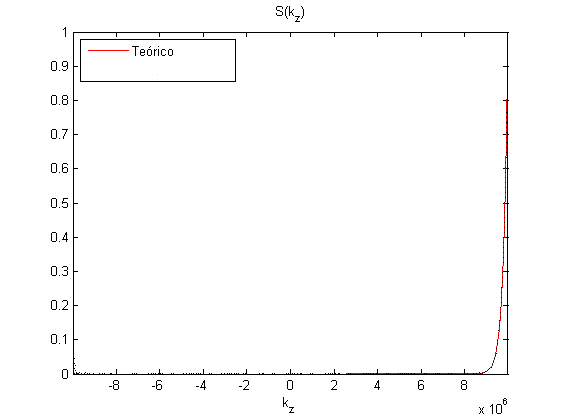
\includegraphics[scale=0.3]{figex1a.png}}
\centering
\subfigure[]{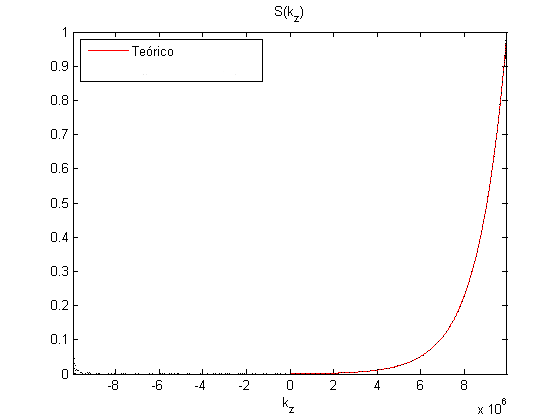
\includegraphics[scale=0.3]{figex2a.png}}\\
\centering
\subfigure[]{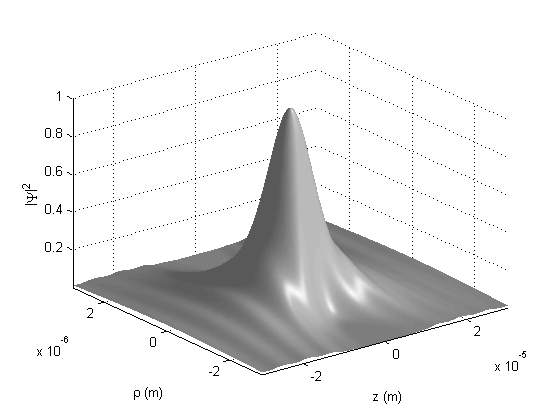
\includegraphics[scale=0.3]{figex1b.png}}
\centering
\subfigure[]{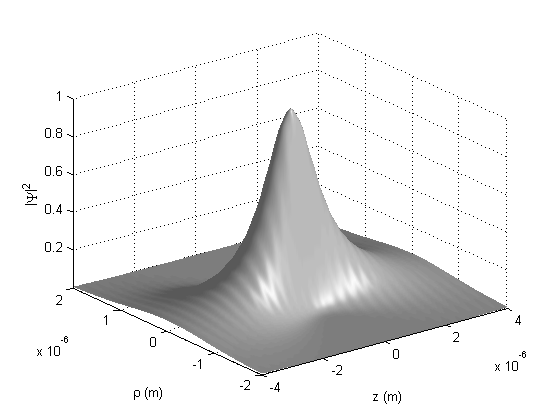
\includegraphics[scale=0.3]{figex2b.png}}\\
\centering
\subfigure[]{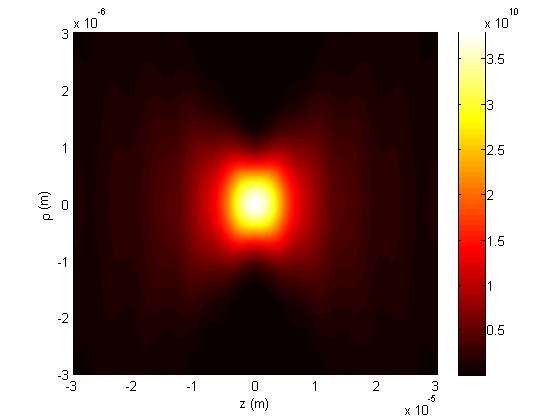
\includegraphics[scale=0.3]{figex1c.png}}
\centering
\subfigure[]{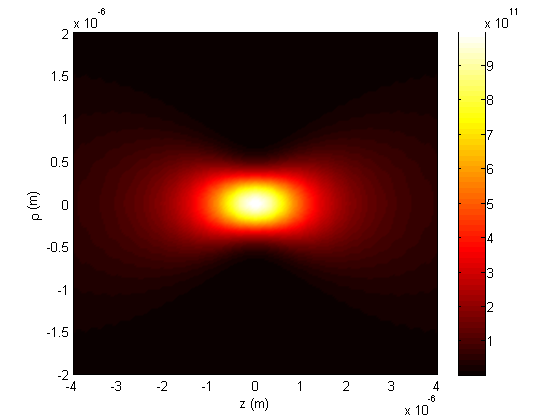
\includegraphics[scale=0.3]{figex2c.png}}\\
\caption{(a)-(b) Gr\'aficos do espectro exponencial paraxial e n\~ao paraxial respectivamente. Os tra\c{c}os em vermelhos representam o espectro dado pela eq. (\ref{e1}). (c)-(d) Padr\~oes de intensidade 3D, solu\c{c}\~oes exatas da equa\c{c}\~ao de onda dos feixes paraxial e n\~ao paraxial respectivamente dados pela eq. (\ref{z4}). (e)-(f) Proje\c{c}\~ao ortogonal da intensidade do feixe exponencial no plano $(\rho,z)$.}
\label{fig1}
\end{figure}
%*******************************************************************************
%*******************************************************************************
Foram analisados dois tipos de espectros: O primeiro, um espectro do tipo paraxial para gerar feixes paraxiais.\\
 Para obter um feixe paraxial, nosso espectro $S(k_z)$ foi concentrado ao redor de $\bar{k}_z = \omega /c=9,97.10^6 m^{-1}$, com $\Delta k_z =1/a = K/100  = 0,199.10^6 m^{-1}\ll \omega /c$ e onde $\Delta k_z/\bar{k}_z=0,02\ll 1$. O gr\'afico te\'orico do espectro paraxial (\ref{e1}) \'e mostrado na Figura \ref{fig1}(a) em cor vermelha.\\
O segundo espectro foi do tipo n\~ao paraxial, com uma largura de banda maior que a primeira $\Delta k_z = 1/a = K/20 = 0,997.10^6 m^{-1}$ e com $\Delta k_z/\bar{k}_z= 0,1$. O gr\'afico do espectro (\ref{e1}) desse segundo caso \'e mostrado na Figura \ref{fig1}(b) em cor vermelha.
Nas figuras \ref{fig1}(c)(d) s\~ao apresentados os padr\~oes de intensidade normalizados em 3D. A Figura \ref{fig1}(c) corresponde ao espectro paraxial obtido da Figura \ref{fig1}(a) e a Figura \ref{fig1}(d) corresponde ao espectro n\~ao paraxial obtido da Figura \ref{fig1}(b). Os feixes obtidos prov\^em de espectros n\~ao paraxiais e paraxiais e s\~ao solu\c{c}\~oes anal\'iticas exatas da equa\c{c}\~ao de onda.\\
Nas Figuras \ref{fig1}(e)(f) s\~ao apresentadas as proje\c{c}\~oes ortogonais das intensidades dos feixes \ref{fig1}(c)(d) no plano $(\rho,z)$. Podemos observar que os feixes produzidos s\~ao propagantes e possuem simetria azimutal.
%*************************************************************************************************************************
\subsection{Espectro quadrado} Seja um espectro quadrado definido por:
\begin{equation}\label{q1}
S(k_{z})= \left\{
\begin{array}{rcl}
     K= 2\omega/c & , & k_{zmin}\leq k_{z}\leq k_{zmax}\\
     0 &  , & $caso contr\'ario$
\end{array}
\right.
\end{equation}
onde $0\leq k_{zmin}\leq k_{zmax}  \leq\omega/c$. A posi\c{c}\~ao do espectro $\bar{k}_z$ e a largura de banda $\Delta k_z=k_{zmax}-k_{zmin}$, determinar\~ao se o espectro quadrado \'e do tipo paraxial ou n\~ao paraxial.\\
Substituindo (\ref{q1}) em (\ref{eqA19}), foram obtidos os coeficientes de Fourier $R_n$ do espectro quadrado $S(k_z)$. Para achar as solu\c{c}\~oes anal\'iticas exatas correspondentes ao espectro quadrado foram substitu\'idos os valores de $R_n$ em (\ref{eqA20}).\\
%*******************************************************************************
%*******************************************************************************
\begin{figure}[h]
\centering
\subfigure[]{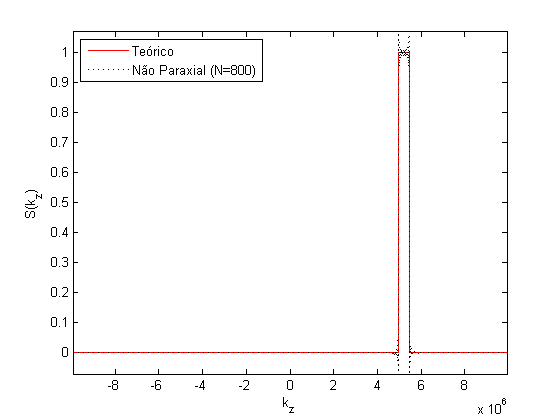
\includegraphics[scale=0.3]{figqu1a.png}}
\centering
\subfigure[]{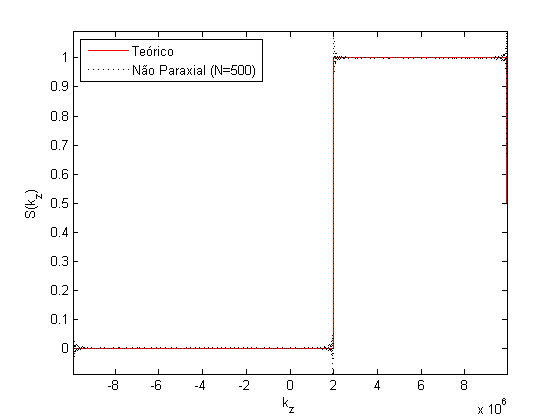
\includegraphics[scale=0.3]{figqu2a.png}}\\
\centering
\subfigure[]{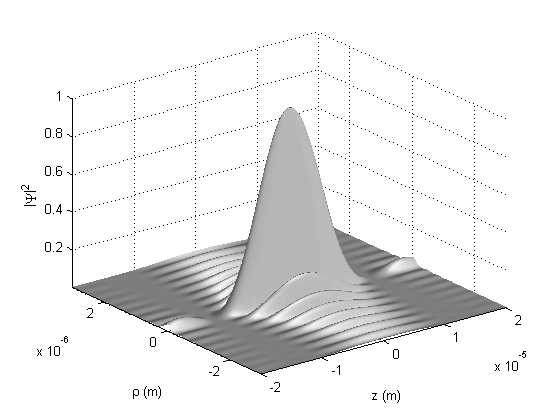
\includegraphics[scale=0.3]{figqu1b.png}}
\centering
\subfigure[]{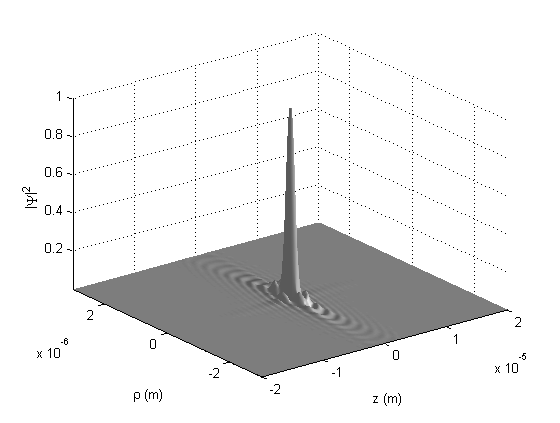
\includegraphics[scale=0.3]{figqu2b.png}}\\
\centering
\subfigure[]{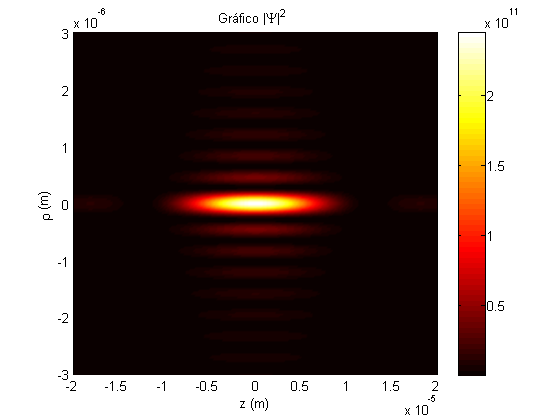
\includegraphics[scale=0.3]{figqu1c.png}}
\centering
\subfigure[]{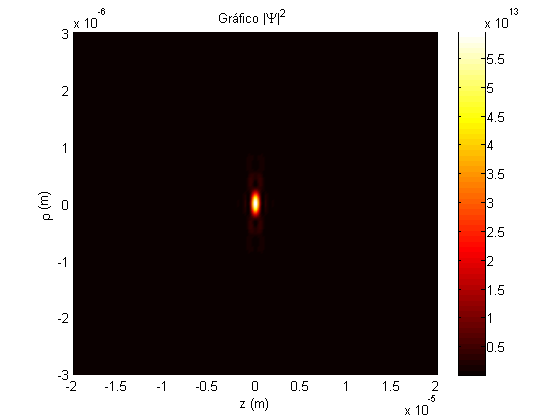
\includegraphics[scale=0.3]{figqu2c.png}}\\
\caption{(a)-(b) Gr\'aficos do espectro quadrado n\~ao paraxial. Os tra\c{c}os em vermelhos representam o espectro dado pela eq. (\ref{q1}). Os tra\c{c}os em cor preta representam a representa\c{c}\~ao de (\ref{q1}) atrav\'es da s\'erie de Fourier dada por (\ref{eqA19}). O n\'umero de termos de coeficientes de Fourier, para os  gr\'aficos foi de 1601 e 1001 respectivamente. (c)-(d) Padr\~oes de intensidade 3D, solu\c{c}\~oes exatas da equa\c{c}\~ao de onda dos feixes n\~ao paraxiais. (e)-(f) Proje\c{c}\~ao ortogonal da intensidade do feixe quadrado no plano $(\rho,z)$.}
\label{fig2}
\end{figure}
%*******************************************************************************
%*******************************************************************************
Foram analisados dois tipos de espectros n\~ao paraxiais.\\
O primeiro, um espectro concentrado em $\bar{k}_z=5,24.10^{6}m^{-1}$ com largura de banda de $\Delta k_z= 4,99.10^{5}m^{-1}$, com $k_{zmin}=4,99.10^{6}m^{-1}$ e $k_{zmax}=5,49.10^{6}m^{-1}$ e com $\Delta k_z/\bar{k}_z=0,095$. O gr\'afico do espectro (\ref{q1}), no primeiro caso, \'e mostrado na Figura \ref{fig2}(a) em cor vermelha, sendo a sua representa\c{c}\~ao atrav\'es da s\'erie de Fourier (\ref{eqA18}) e mostrada em cor preta. O n\'umero total de coeficientes de Fourier usado foi de $1601$, ou seja $N=800$.\\
O segundo espectro foi para uma largura de banda maior que a primeira $\Delta k_z= 7,98.10^{6}m^{-1}$ concentrado em $\bar{k}_z=5,99.10^{6}m^{-1} $, com $k_{zmin}=1,99.10^{6}m^{-1}$ e $k_{zmax}=9,98.10^{6}m^{-1}$, e com $\Delta k_z/\bar{k}_z=1,332$. O gr\'afico do espectro (\ref{q1}) desse segundo caso \'e mostrado na Figura \ref{fig2}(b) em cor vermelha, sendo a sua representa\c{c}\~ao atrav\'es da s\'erie de Fourier (\ref{eqA18}) \'e mostrada em cor preta. O n\'umero total de coeficientes de Fourier usado para este \'ultimo espectro foi de $1001$, ou seja $N=500$.\\
Na Figura \ref{fig2}(c)-(d) s\~ao apresentados os padr\~oes de intensidade em 3D. A Figura \ref{fig2}(c) corresponde ao espectro n\~ao paraxial obtido da Figura \ref{fig2}(a) e a Figura \ref{fig2}(d) corresponde a um espectro menos concentrado, obtido da Figura \ref{fig2}(b). Pode-se observar que o espectro mais concentrado (Figura \ref{fig2}(a)) produz uma maior propaga\c{c}\~ao do feixe. Os feixes produzidos possuem simetria azimutal.\\
Na Figura \ref{fig2}(e)-(f) s\~ao apresentadas as proje\c{c}\~oes ortogonais das intensidades dos feixes no plano $(\rho,z)$.  Os feixes obtidos prov\^em de espetros n\~ao paraxiais e s\~ao solu\c{c}\~oes anal\'iticas exatas da equa\c{c}\~ao de onda.\\
Para um espectro com largura de banda de $\Delta k_z=4,99.10^{6}m^{-1}$, o feixe n\~ao paraxial tem um spot com raio inicial igual a $0,4.10^6m$ aproximadamnete e uma profundidade de campo de $10,0.10^{-6}$m (Figura $\ref{fig2}$(e)). Para um espectro com largura de banda maior de $\Delta k_z=7,98.10^{6}m^{-1}$ , o raio do spot \'e de tamb\'em de $0,4.10^6m$ e a profundidade do campo do feixe n\~ao paraxial \'e de $0,1.10^{-5}$m (Figura $\ref{fig2}$(f)). Portanto, o feixe com espectro mais concentrado (Figura \ref{fig2}(a)), menor largura de banda, possui uma profundidade maior em rela\c{c}\~ao ao feixe menos concentrado (Figura \ref{fig2}(b)). Repare tamb\'em que os raios dos spots dos feixes produzidos s\~ao do ordem do comprimento de onda ($\lambda = 0,632.10^6m$), o qual caracteriza um feixe n\~ao paraxial.  
%**************************************************************************************************************************
\subsection{Espectro gaussiano} Seja um espectro gaussiano definido por:
\begin{equation}\label{ga1}
S(k_{z})= \left\{
\begin{array}{rcl}
  2(\omega/c)\exp(-a(k_z - \bar{k}_z)^2) & , & 0\leq k_{z}\leq \omega/c\\
     0 &  , & $caso contr\'ario$
\end{array}
\right.
\end{equation}
Onde $\bar{k}_z$ indica a posi\c{c}\~ao do centro do espectro. A largura de banda $\Delta k_z$ do espectro \'e diretamente proporcional ao valor do desvio padr\~ao $1/\sqrt{(2a)}$, o qual determina se o espectro gaussiano\'e do tipo paraxial ou n\~ao paraxial.  \\
Substituindo (\ref{ga1}) em (\ref{eqA19}), foram obtidos os coeficientes de Fourier $R_n$ do espectro gaussiano $S(k_z)$. Para obter as solu\c{c}\~oes anal\'iticas exatas correspondentes ao espectro gaussiano foram substitu\'idos os valores de $R_n$ em (\ref{eqA20}).\\
%*******************************************************************************
%*******************************************************************************
\begin{figure}[h]
\centering
\subfigure[]{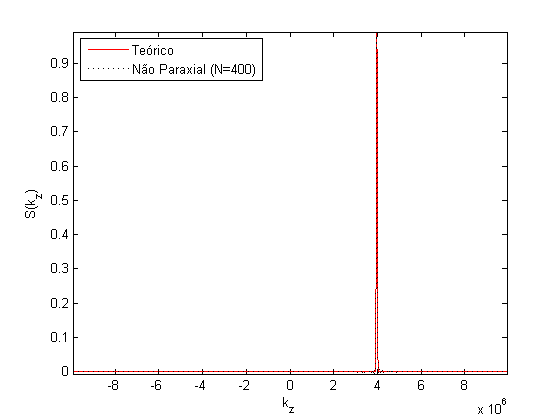
\includegraphics[scale=0.3]{figgau1a.png}}
\centering
\subfigure[]{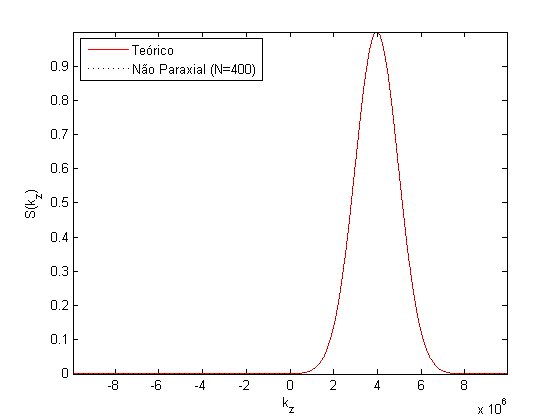
\includegraphics[scale=0.3]{figgau2a.png}}\\
\centering
\subfigure[]{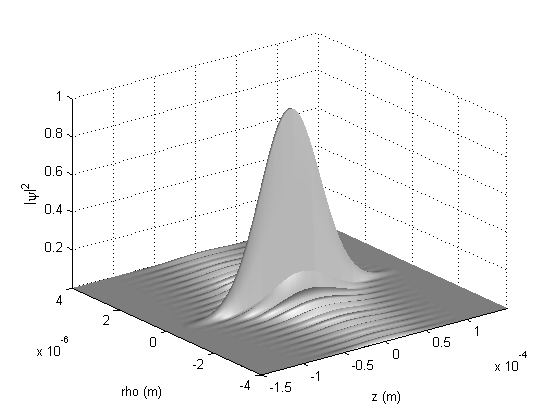
\includegraphics[scale=0.3]{figgau1b.png}}
\centering
\subfigure[]{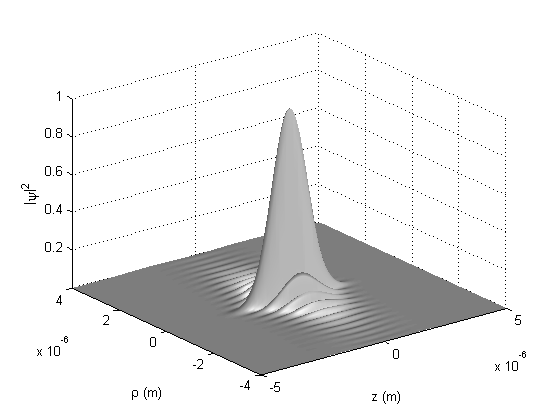
\includegraphics[scale=0.3]{figgau2b.png}}\\
\centering
\subfigure[]{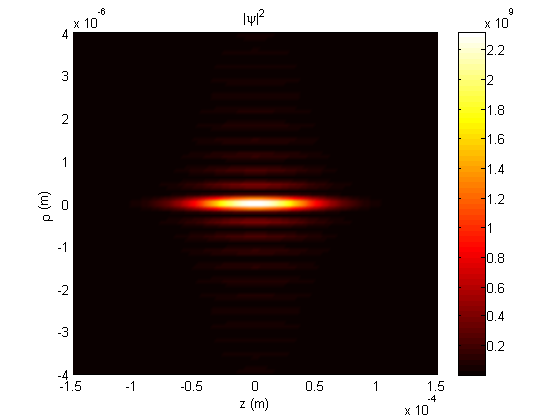
\includegraphics[scale=0.3]{figgau1c.png}}
\centering
\subfigure[]{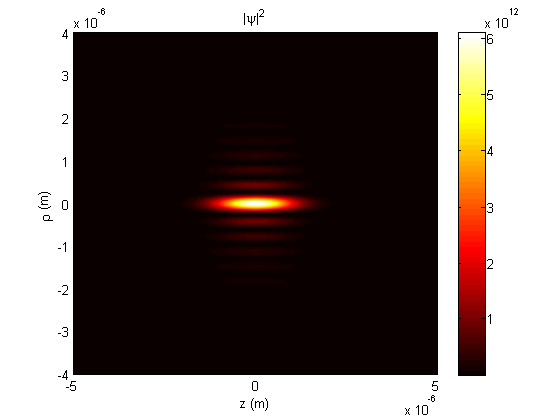
\includegraphics[scale=0.3]{figgau2c.png}}\\
\caption{(a)-(b) Gr\'aficos do espectro gaussiano n\~ao paraxial concentrado e n\~ao concentrado respectivamente. Os tra\c{c}os em vermelhos representam o espectro dado pela eq. (\ref{ga1}). Os tra\c{c}os em cor preta representam a representa\c{c}\~ao de (\ref{ga1}) atrav\'es da s\'erie de Fourier dada por (\ref{eqA19}). O n\'umero de termos de coeficientes de Fourier, para os  gr\'aficos foi de 801. (c)-(d) Padr\~oes de intensidade 3D, solu\c{c}\~oes exatas da equa\c{c}\~ao de onda dos feixes n\~ao paraxiais. (e)-(f) Proje\c{c}\~ao ortogonal da intensidade do feixe quadrado no plano $(\rho,z)$.}
\label{fig3}
\end{figure}
%*******************************************************************************
%*******************************************************************************
Do mesmo jeito dos itens anteriores foram analisados dois tipos de espectros n\~ao paraxiais.\\
O primeiro, um espectro $S(k_z)$ concentrado ao redor de $\bar{k}_z = 0,4\omega /c=3,97.10^6 m^{-1}$, com o desvio padr\~ao $1,99.10^{4}m^{-1}$ ($a=5,0.10^5/K^2$) e com $\Delta k_z/\bar{k}_z=0,005$. O gr\'afico do espectro (\ref{ga1}), no primeiro caso, \'e mostrado na Figura \ref{fig3}(a) em cor vermelha, sendo a sua representa\c{c}\~ao atrav\'es da s\'erie de Fourier (\ref{eqA18}) e mostrada em cor preta. O n\'umero total de coeficientes de Fourier usado foi de $801$, ou seja $N=800$.\\
O segundo espectro foi para uma largura de banda maior que a primeira $9,93.10^{5}m^{-1}$ ($a=200/K^2$) e com $\Delta k_z/\bar{k}_z=0,250$. O gr\'afico do espectro (\ref{ga1}) desse segundo caso \'e mostrado na Figura \ref{fig3}(b) em cor vermelha, sendo a sua representa\c{c}\~ao atrav\'es da s\'erie de Fourier (\ref{eqA18}) \'e mostrada em cor preta. O n\'umero total de coeficientes de Fourier usado para este \'ultimo espectro foi de $801$, ou seja $N=400$.\\
Na Figura \ref{fig3}(c)-(d) s\~ao apresentados os padr\~oes de intensidade em 3D. A Figura \ref{fig3}(c) corresponde ao espectro n\~ao paraxial concentrado obtido da Figura \ref{fig3}(a) e a Figura \ref{fig3}(d) corresponde a um espectro n\~ao paraxial n\~ao concentrado, obtido da Figura \ref{fig3}(b). Pode-se observar que quanto mais estreito \'e o espectro, maior ser\'a a profundidade de campo do feixe resultante.\\
Na Figura \ref{fig3}(e)-(f) s\~ao apresentadas as proje\c{c}\~oes ortogonais das intensidades dos feixes no plano $(\rho,z)$.  Os feixes obtidos prov\^em de espetros n\~ao paraxiais e s\~ao solu\c{c}\~oes anal\'iticas exatas da equa\c{c}\~ao de onda.\\
O espectro maior concentrado $1,99.10^{4}m^{-1}$ produz um feixe n\~ao paraxial com alcance de $1,0.10^{-4}$m (Figura $\ref{fig3}$(e)). Para um espectro menos concentrado $9,93.10^{5}m^{-1}$, o alcance do feixe n\~ao paraxial \'e de $2,0.10^{-6}$m (Figura $\ref{fig3}$(f)). Portanto, o feixe com espectro mais concentrado (Figura \ref{fig3}(a)), menor largura de banda, possui uma profundidade maior em rela\c{c}\~ao ao feixe menos concentrado (Figura \ref{fig3}(b)). Se fizemos  a largura de nossa gaussiana tender a zero, teremos como resultado um feixe de bessel, que possui concentra\c{c}\~ao do campo transversal e profundidade de campo infinita, portanto fluxo de pot\^encia infinito .  
%**************************************************************************************************************************
\section{Feixes Escalares puramente propagantes sem simetria azimutal}
Outro analise interessante \'e a obten\c{c}\~ao de de feixes n\~ao paraxiais sem simetria azimutal como solu\c{c}\~oes anal\'iticas exatas da equa\c{c}\~ao de onda. Feixes sem simetria azimutal podem ser constru\'idos como superposi\c{c}\~oes de fun\c{c}\~oes de Bessel de $\nu-$ordem, onde $\nu$ \'e um inteiro positivo. Do mesmo jeito que na obten\c{c}\~ao de feixes escalares n\~ao  paraxiais, os feixes sem simetria azimutal s\~ao complicados de obter devido \`a complexidade da integral neste caso, a integral em (\ref{eq11}). A seguir usaremos o mesmo m\'etodo matem\'atico usado anteriormente na obten\c{c}\~ao de feixes n\~ao paraxiais para solucionar (\ref{eq11}) e, portanto, fornecer solu\c{c}\~oes anal\'iticas exatas descrevendo feixes n\~ao paraxiais (e tamb\'em paraxiais) sem simetria azimutal puramente propagantes.\\
Partimos do feixe com simetria azimutal ($\psi(\rho,z,t)$) dado em (\ref{eqA20}), com espectro exponencial ($S(k_z)$) dado em (\ref{e1}). Usando (\ref{eq6}) obtemos um novo feixe sim simetria azimutal ($\psi_{1}(\rho,\phi,z,t)$) o qual \'e uma solu\c{c}\~ao exata da equa\c{c}\~ao de onda:
\begin{eqnarray}\label{eqs1}
\psi_{1}(\rho,\phi,z,t) &=& \frac{\partial\psi }{\partial \rho}\exp[{\rm i}\phi]\nonumber\\
\psi_{1}(\rho,\phi,z,t) &=&  \exp[-{\rm i}\omega t]\exp[{\rm i}\phi]\left( \frac{w^2}{c^2}\right)\sum\limits_{n=-\infty}^{\infty}R_n \rho  \left(\frac{\cos [h]}{h^2}-\frac{\sin [h]}{h^3}\right)
\end{eqnarray}
onde 
\begin{equation}\label{eqs2}
  R_n=\frac{1}{K}\int_{-\omega/c}^{\omega/c} S(k_z)\exp[-{\rm i}\frac{2\pi}{K}n k_z]dk_z
\end{equation}
\begin{equation}\label{eqs3}
h = \sqrt{\frac{\omega^2}{c^2}\rho^2+(z\frac{\omega}{c}+\pi n)^2}
\end{equation}
%*******************************************************************************
%*******************************************************************************
\begin{figure}[h]
\centering
\subfigure[]{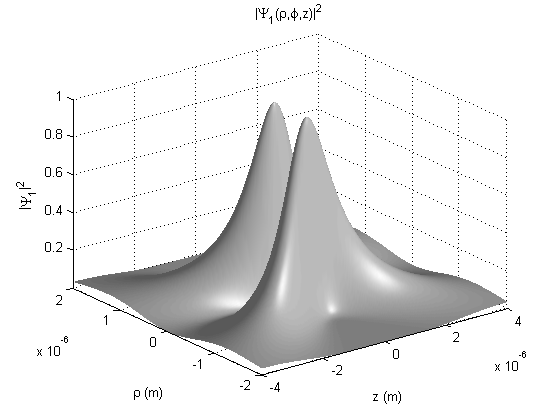
\includegraphics[scale=0.35]{figexSS1a.png}}
\centering
\subfigure[]{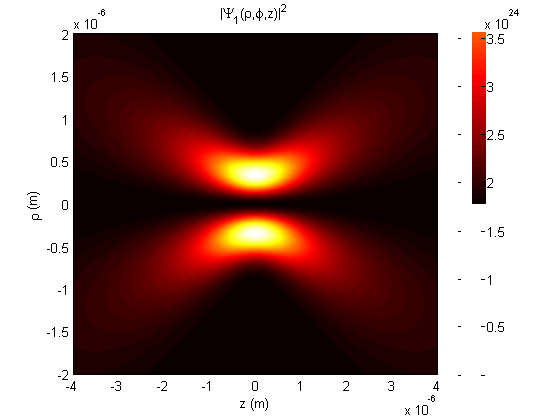
\includegraphics[scale=0.35]{figexSS1b.png}}
\centering
\subfigure[]{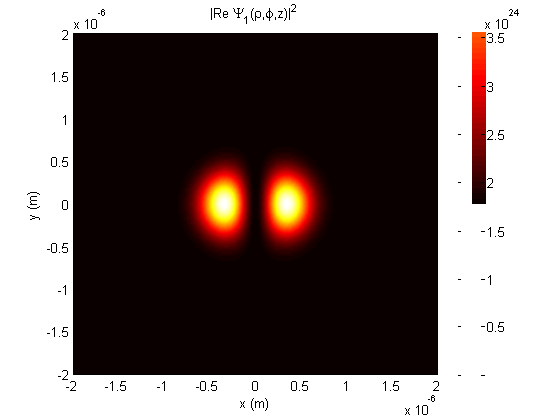
\includegraphics[scale=0.35]{figexSS1c.png}}
\caption{(a) Padr\~ao de intensidade 3D, solu\c{c}\~oes exatas da equa\c{c}\~ao de onda dos feixes n\~ao paraxiais sem simetria azimutal do espectro exponencial (\ref{e1}) para $\nu=1$. (b) Proje\c{c}\~ao ortogonal da intensidade do feixe quadrado no plano $(\rho,z)$. (c) Proje\c{c}\~ao ortogonal da parte real do feixe exponencial no plano $(x,y)$ para $z=0$.}
\label{fig4}
\end{figure}
%*******************************************************************************
%*******************************************************************************
Reparamos que a solu\c{c}\~ao exata (\ref{eqs1}) corresponde \`a superposi\c{c}\~ao dada em (\ref{eq11}), com $S^{'}(k_z)=S(k_z)(-k_{\rho})$, onde $S(k_z)$ esta dado por (\ref{e1}).\\
Foi analisado o espectro exponencial do tipo n\~ao paraxial ($S(k_z)$), com uma largura de banda $\Delta k_z = a = 100/K = 5,01.10^6 m^{-1}$. O gr\'afico do espectro (\ref{e1}) desse caso \'e mostrado na Figura \ref{fig1}(b) em cor vermelha, sendo a sua representa\c{c}\~ao atrav\'es da serie de Fourier (\ref{eqA18}) e mostrada em cor preta. O n\'umero total de coeficientes de Fourier usado foi de $801$, ou seja $N=400$.\\
Na figura \ref{fig4}(a) \'e apresentado o padr\~ao de intensidade normalizados em 3D. Notar que a Figura \ref{fig4}(a) corresponde ao espectro n\~ao paraxial $S^{'}(k_z)=S(k_z)(-k_{\rho})$, onde $S(k_z)$ \'e obtido da Figura \ref{fig1}(b). O feixe obtido prov\^e do espectro n\~ao paraxial e \'e solu\c{c}\~ao anal\'itica exata da equa\c{c}\~ao de onda. Podemos observar que o feixe produzido \'e propagante e n\~ao possui simetria azimutal ($\nu=1$).\\
Na Figura \ref{fig4}(b) \'e apresentada a proje\c{c}\~ao ortogonal da intensidade do feixe \ref{fig4}(a) no plano $(\rho,z)$ e na Figura \ref{fig4}(c) \'e apresentada a proje\c{c}\~ao ortogonal do quadrado da parte real do feixe \ref{fig4}(a) no plano $(x,y)$, com $z=0$. 
%*************************************************************************************************************************

\chapter{Resultados Parciais: Segunda contribui\c{c}\~ao}

\section{Feixes Vectoriais puramente propagantes com simetria azimutal}

\subsection{Metodologias matem\'aticas para a constru\c{c}\~ao de feixes vetoriais}
Um feixe electromagn\'etico pode-se
\chapter{Plano de trabalho e cronograma}
O propósito deste capítulo é apresentar as etapas necessárias para a realização desde trabalho.\\
O cronograma de atividades com resolução bimestral é mostrado na Tabela (\ref{tab1}), o qual descreve a programação das atividades já realizadas e as previstas até o término da dissertação. O número $1$ marca a data da atividade e o número $0$ indica que não há atividade. O número 1 riscado indica que a atividade j foi realizada.\\

\begin{table}[h]
\caption{Cronograma de actividades} %title of the table
\centering
% centering table
\begin{tabular}{c rrrrrr}
% creating eight columns
\hline\hline
%inserting double-line
 &\multicolumn{6}{c}{2012} \\ [0.5ex]
\hline
% inserts single-line
 Temas / Tempo & Jan/Fev & Mar/Abr & Mai/Jun & Jul/Ago & Set/Out & Nov/Dez\\
\hline
\centering
% Entering row contents
Pesquisa bibliogr\'afica & \cancel{1} & 0 & 0 & 0 & 0 & 0\\
Feixes escalares  & \cancel{1} & \cancel{1} & 0 & 0 & 0 & 0\\
Feixes sim simetria & 0 & \cancel{1} & \cancel{1} & 0 & 0 & 0\\
Analice vetorial Met 1&  0 & 0 & \cancel{1} & 1 & 0 & 0\\
Analice vetorial Met 2&  0 & 0 & 0 & 0 & 1 & 0\\
Prepara\c{c}\~ao da diserta\c{c}\~ao &  0 & 0 & 0 & 0 & 1 & 1\\[1ex] % [1ex] adds vertical space
\hline

% inserts single-line
\end{tabular}
\label{tab1}
\end{table}
Iniciamos o plano de trabalho com a pesquisa bibliográfica, a qual também inclui o estudo de feixes escalares e vetoriais propagantes paraxiais e não paraxiais com simetria azimutal os quais foram mostrados no capítulo 2. Neste período estudou-se a metodologia matemática proposta em \cite{Lya:2}, desenvolvida para fornecer soluções analíticas exatas da equação de onda. O método matemático desenvolvido em (\cite{Lya:2}) para a obtenção de feixes escalares não paraxiais sem simetria azimutal é também abordado neste período.\\
Na Tabela (\ref{tab1}) mostramos a continuação do plano de trabalho. A metodologia matemática proposta para a obtenção de feixes escalares e vetoriais foi exposta no capítulo $3$ e $4$, assim como os resultados já obtidos para os feixes escalares com e sem simetria azimutal. No capítulo $4$ também mostramos os resultados obtidos para o caso vetorial mediante o método das derivadas parciais. Nos próximos meses continuaremos com o analise vetorial dos feixes eletromagnéticos com a obtenção de novas e interessantes polarizações.\\
Nosso cronograma ser\'a finalizado com a preparação da dissertação de acordo com as diretrizes do programa de pós-graduação da FEEC-UNICAMP.
\subsection*{Submissões}
At\'e o presente momento, foi realizada a submissão de um artigo para o congresso, o qual foi aceito e estamos finalizando um artigo para ser submetido a um periódico internacional. O artigo submetido e aceito no congresso de MOMAG foi:

\begin{itemize}
\item R. L. Garay-Avendaño and M. Zamboni-Rached, "Feixes Não Paraxiais: Uma Formulação Analítica Exata. I. A Teoria Escalar", aceito no $15^{o}$ Simpósio Brasileiro de Microondas e Optoeletrônica e $10^o$ Congresso Brasileiro de Eletromagnetismo, João Pessoa, PA, Brasil (2012).
\end{itemize}  

%-------------------------------
%\chapter{Conclus\~{o}es e Perspectivas}
%\section*{Perspectivas}
%\subsection*{Publica\c{c}\~{o}es}
\chapter{Conclus\~oes Parciais}

Neste trabalho, apresentamos um m\'etodo te\'orico capaz de de 
proporcionar solu\c{c}\~oes anal\'iticas exatas da equa\c{c}\~ao 
de onda, para qualquer tipo de espectro $S(k_z)$. As solu\c{c}\~oes 
encontradas correspondem a feixes escalares (propagantes) n\~ao paraxiais 
com simetria azimutal. Esses resultados s\~ao importantes pois al\'em de 
fornecerem solu\c{c}\~oes anal\'iticas exatas, evitam demoradas 
simula\c{c}\~oes num\'ericas.
 % Conclusões


%=============================== Bibliografia =================================================
\addcontentsline{toc}{chapter}{Bibliografia}
\renewcommand{\bibname}{Bibliografia}
\markboth{Bibliografia}{Bibliografia}

\bibliographystyle{dcu}
\bibliography{meubib}


\end{document}
